\documentclass[12pt,french]{article}
\input preambule_2013

\begin{document}
\begin{center}
\psframebox{%
\parbox{0.98\linewidth}{
        \centering\bfseries\Large
        Accompagnement personnalisé \\
        Des notions importantes pour les autres disciplines
}}
\end{center}\bigskip
    
    Paul souhaiterait construire une piscine dans son jardin de $0,5~hm^2$.\par
    Il va voir un artisan qui lui propose de construire une piscine de longueur $L = 15~m$, de largeur $\ell = 5~m$ et de profondeur $p = 2~m$.
    
    \begin{enumerate}
        \item Paul estime que la surface du terrain est suffisante pour construire une telle piscine.\par Expliquer pourquoi.
    \end{enumerate}

    Les quatre murs de la piscine seront chacun recouverts de carrelage. Un carreau du carrelage est de forme carrée de $50~cm$ de côté.
    
    \begin{enumerate}[resume]
        \item Combien faudra-t-il de carreaux pour recouvrir l'intégralité des quatre murs de la piscine ?
    \end{enumerate}
    
    L'artisan explique à Paul que la piscine ne peut pas être complètement remplie. Au maximum, on ne peut remplir qu'à $95\%$ du volume total.
    
    \begin{enumerate}[resume]
        \item Quelle quantité d'eau maximale Paul pourra-t-il mettre dans sa piscine ? \par Donner le résultat en $m^3$ puis en $L$.
    \end{enumerate}
    
    Le sol de la piscine sera recouvert d'un revêtement spécial vendu dans des pot. Un pot permet de recouvrir une surface de $3~m^2$ et coûte \EUR{$45$}.\par
    Le carrelage est vendu par paquet de $10$ carreaux. Un paquet coûte \EUR{$72,50$}.\par
    L'eau coûte \EUR{$6$} par $m^3$.\par
    Et enfin, Paul doit prévoir un budget supplémentaire de \EUR{$\np{16580}$} pour la préparation du terrain, la construction de la piscine et la main d'{\oe}uvre.
    
    \begin{enumerate}[resume]
        \item Combien devra payer Paul au total sachant qu'il remplit la piscine au maximum autorisé.
    \end{enumerate}
    
    L'entrepreneur accepte de faire une remise de \EUR{$\np{1260}$}.
    
    \begin{enumerate}[resume]
        \item À quel pourcentage du total correspond cette remise ? Arrondir à l'unité.
    \end{enumerate}
    
    Finalement, Paul décide que la piscine aura une profondeur de $1~m$ d'un côté et que le sol descendra progressivement en pente douce jusqu'à atteindre la profondeur de $2~m$ comme indiqué sur la figure ci-dessous.\medskip
    
    \begin{center}
        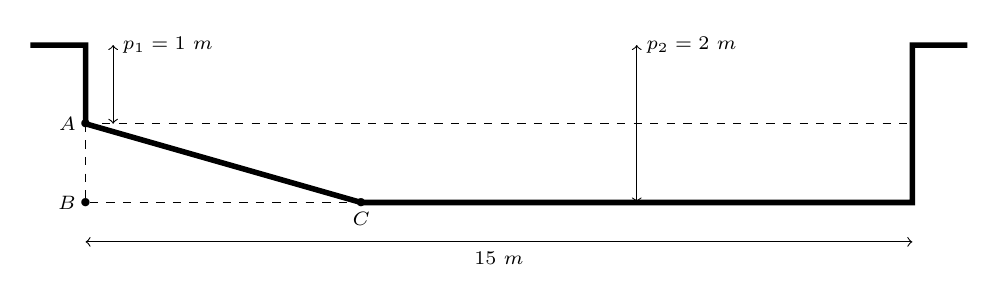
\begin{tikzpicture}[x=0.7cm]
            \draw[line width=2pt] (-1,0) -- (0,0) -- (0,-1) -- (5,-2) -- (15,-2) -- (15,0) -- (16,0);
            \draw[dashed] (0,-1) -- (15,-1);
            \draw[<->] (10,0) -- (10,-2);
            \draw (10,0) node[right] {\scriptsize $p_2=2~m$};
            \draw[<->] (0.5,0) -- (0.5,-1);
            \draw (0.5,0) node[right] {\scriptsize $p_1=1~m$};
            \draw[dashed] (0,-1) node {\scriptsize $\bullet$} node[left] {\scriptsize $A$} --
                                   (0,-2) node {\scriptsize $\bullet$} node[left] {\scriptsize $B$} --
                                   (5,-2) node {\scriptsize $\bullet$} node[below] {\scriptsize $C$};
            \draw[<->] (0,-2.5) -- (15,-2.5) node[below,midway] {\scriptsize $15~m$};
        \end{tikzpicture}
    \end{center}
    
    \begin{enumerate}[resume]
        \item Le triangle $ABC$ est rectangle en $B$.
                \begin{enumerate}
                    \item Paul souhaiterait que la longueur $BC$ soit égale à $5~m$. Combien doit alors mesurer l'angle $\widehat{ACB}$ ? Arrondir à l'unité.
                    \item Pour des raisons de construction, l'angle $\widehat{BAC}$ mesurera finalement $82\degres$. Quelle sera alors la longueur du segment $[AC]$ ?
                \end{enumerate}
    \end{enumerate}
\end{document}


    